\section{Subspace Clustering}
The overall idea of subspace clustering is to identify the subspaces that allows better clustering than the entire space $\mathcal{S}$. Two different approaches of subspace clustering will be discussed in this section including three subspace clustering algorithms. All three is bottom-up approaches meaning they must implement the monotonicity property \cite[p.~1:11]{kriegel-2009}, see Lemma \ref{lem:mono}.

\subsection{Grid-Based approach}
In a grid-based approach, $\mathcal{S}$ is partitioned into an axis-parallel grid structure. Each grid cell forms a axis-parallel, hyper-rectangular \textit{unit}, and the number of points within each unit is counted. This process is initially applied in the 1-dimensional space for each attribute. Units that contain a number of points exceeding a predefined \textit{density threshold} are retained as \textit{dense units} (DUs). Then, these DUs are merged with adjacent ones in the next level (2-dimensional space) to form \textit{candidate dense units} (CDUs), those of which are actually dense are kept. The final DUs are then the clusters found by the algorithm which will be described using minimal representations in the form of \textit{Disjunctive Normal Form} (DNF) expressions using intervals of the attributes. Two algorithms that follows this approach are CLIQUE and MAFIA.

\subsubsection{CLIQUE}
is the first proposed subspace clustering methods using a grid-based approach. It starts, by partitioning $\mathcal{S}$ into equal-sized \textit{windows} (or \textit{units}) of width $\varepsilon$ (input parameter). Then, DUs are identified in for the 1-dimensional case, by counting the number of points in each window, for example, using a histogram, as shown in Figure \ref{fig:dense_cells_and_regions}, where each window has a certain \textit{bin} count. For example, if $\varepsilon = 0.2$, then 3 DUs are identified in $A_1$, while 4 DUs are identified in $A_2$. The total of 7 DUs identified in the 1-dimensional space, will then be used to form CDUs in the 2-dimensional space. Specially, CLIQUE uses the following definition to form CDUs in $k$-dimensional space:
\begin{definition}\label{def:cdu_clique}
    CDUs in $k$-dimensional space are formed by merging DUs from the $(k-1)$-dimensional space that share the \textit{first} $(k-2)$ attributes.
\end{definition}\todo{måske gøre det klart at det ikke har noget med Apriori at gøre.}
We denote Definition \ref{def:cdu_clique} as the \textit{first-approach}. Having formed the CDUs, then as mentioned, only the CDUs that are actually dense are kept for further processing.

To optimize performance, CLIQUE applies a pruning technique to the subspaces by calculating their \textit{coverage}. Subspaces with low coverage (i.e., those containing few points) are pruned to reduce computation time. This approach helps manage the potentially large number of CDUs that CLIQUE may generate. However, this pruning strategy carries the risk of removing subspaces that might contain valuable cluster information.

Once the final DUs have been identified, CLIQUE seeks to group these DUs into clusters. A \textit{region} is formed when adjacent DUs are connected within a subspace. A \textit{maximal region} is the largest set of connected DUs that cannot be expanded further by adding more adjacent DUs. These maximal regions represent the extent of a cluster in the given subspace. For instance, in Figure \ref{fig:dense_cells_and_regions}, two distinct maximal regions, labeled $A$ and $B$, are shown. The minimal cover for the cluster has the following DNF expression: $((0.2 \leq A_1 < 0.6) \land (0.4 \leq A_2 < 0.8)) \lor ((0.4 \leq A_1 < 0.8) \land (0.2 \leq A_2 < 0.6))$.
\begin{figure}[H]
    \vspace*{-0.7cm}
    \centering
    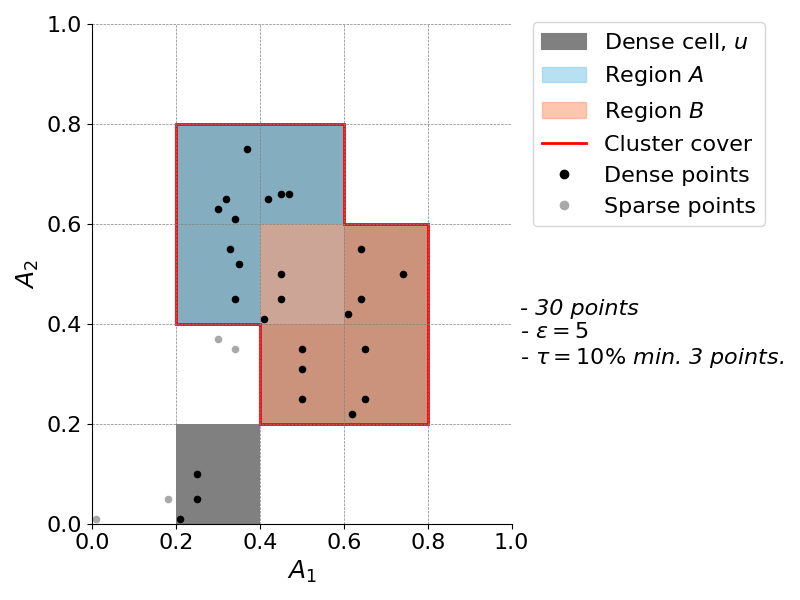
\includegraphics[width=0.4\textwidth]{figures/dense_cells_and_regions.png}
    \caption{2-dimensional space containing 2 overlapping dense regions with 8 DUs in total.}
    \label{fig:dense_cells_and_regions}
    \vspace*{-0.7cm}
\end{figure}

\subsubsection{MAFIA}
can be seen as an extension to CLIQUE and follows mostly the same procedure. However, MAFIA has the following changes:
\begin{enumerate}
    \item Automatically determined variable sized grids based on the data distribution.
    \item Forms CDUs using all combinations of the dimensions that the DUs contains.
    \item Do not use the pruning technique as it could result in lost information, as already noted in \cite{clique}.
    \item Tries to parallelize the clustering process for higher performance.
\end{enumerate}
Point 1 and 2 will in the following be explained in more detail.

\paragraph{The Adaptive Grid Algorithm}
starts by divide each attribute into high $n$-number of equal-sized windows (default $n = 1000$). Then, from left to right, two windows are merged together if their bin count are within a percentage of difference $\beta$ (input parameter). That means, a high $\beta$ value result in many merged windows, and vice-versa. If two windows are merged together, the highest bin count are assigned to the window, meaning the bin count that should be used to be compared with the next window. In other words, the algorithm does not use the total bin count of the two for the next comparison. Figure \ref{fig:adaptive_grids} shows an example before and after running the Adaptive algorithm using different values of $\alpha$ and $\beta$. Having merged the windows, the algorithm finally determines a \textit{dense-level} for each of the windows, that determines how many points a window must contain for a unit to be dense, thus determines whether it should be a CDU for higher dimensional spaces. The dense-level is given by: $\text{dense-level} = \frac{\alpha \cdot a\cdot |\mathcal{D}|}{D_i}$, where $a$ is the \textit{size} of the window, $\alpha$ is the \textit{cluster dominance factor} (input parameter) and $D_i$ is the \textit{total range} $A_i$ covers. Thus, a higher $\alpha$ results in a higher dense-level, and vice-versa, as seen in Figure \ref{fig:adaptive_grids}.
\begin{figure}[H]
    \vspace*{-0.7cm}
    \centering
    \subfloat[][Before Adaptive.]{%
        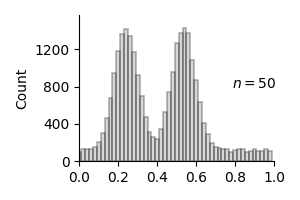
\includegraphics[width=0.24\textwidth]{figures/adaptive_grids/before_adaptive}\label{fig:adaptive_grids_before}}~
    \subfloat[][After Adaptive, $\alpha = 1.5$, $\beta = 20\%$.]{%
        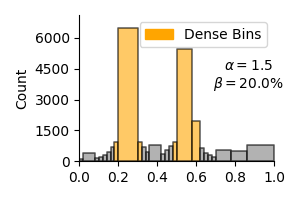
\includegraphics[width=0.24\textwidth]{figures/adaptive_grids/after_adaptive_alpha_1.5_beta_0.2.png}\label{fig:after_adaptive_alpha_1.5_beta_0.2}}~
    \subfloat[][After Adaptive, $\alpha = 2$, $\beta = 20\%$.]{%
        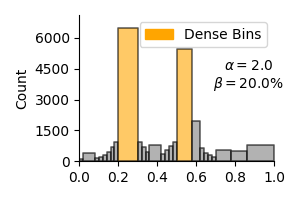
\includegraphics[width=0.24\textwidth]{figures/adaptive_grids/after_adaptive_alpha_2.0_beta_0.2.png}\label{fig:after_adaptive_alpha_2.5_beta_0.2}}~
    \subfloat[][After Adaptive, $\alpha = 2$, $\beta = 30\%$.]{%
        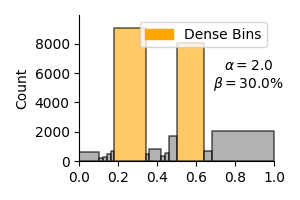
\includegraphics[width=0.24\textwidth]{figures/adaptive_grids/after_adaptive_alpha_2.0_beta_0.3.png}\label{fig:after_adaptive_alpha_2.5_beta_0.3}}~
    \caption{Illustration of the effect of adaptive grids.}
    \label{fig:adaptive_grids}
    \vspace*{-0.7cm}
\end{figure}

\paragraph{The CDU Generation of MAFIA}
is slightly different compared to CLIQUE. MAFIA uses the following definition when forming CDUs in $k$-dimensional space:
\begin{definition}\label{def:cdu_mafia}
    CDUs in $k$-dimensional space are formed by merging DUs from the $(k-1)$-dimensional space that share \textit{any} $(k-2)$ attributes.
\end{definition}
We denote Definition \ref{def:cdu_mafia} as the \textit{any-approach}. The difference between CLIQUE's \textit{first-approach} and MAFIA's \textit{any-approach} is that MAFIA explores any combination of dimensions that the DUs may share. Indeed, the \textit{any-approach} could result in many combinations, and in fact the worst case running time is as high as $O(Ndu^2)$, where $Ndu$ is the number of DUs. MAFIA can afford this high running time as it uses adaptive grids which reduces the number of generated DUs. Actually, CLIQUE also could implement the \textit{any-approach}, however, big grid sizes may then be required to ensure few DUs are generated. Also note that, the \textit{any-approach} can produce repeated CDUs, which therefore needs to be eliminated before proceeding to higher dimensions. Table \ref{tab:cdu} illustrates the advantage of the \textit{any-approach}. Here, 3 DUs are provided to the a 4-dimensional space. Both CLIQUE and MAFIA would form a 4-dimensional CDU based on DU1 and DU2, as they share the \textit{first} two dimensions. However, only MAFIA would form a CDU based on DU1 and DU3.
\begin{table}[H]
    \vspace*{-0.7cm}
    \centering
    \begin{tabular}{l|c|c|c|}
                        & DU1           & DU2           & DU3           \\ \hline
        Dim. used by DU & $\{1, 2, 3\}$ & $\{1, 2, 4\}$ & $\{2, 3, 4\}$ \\
    \end{tabular}
    \vspace*{0.2cm}
    \caption{Illustration showing the difference of CDU generation of CLIQUE and MAFIA. The resulting CDUs are used in the 4-dimensional space.}
    \label{tab:cdu}
    \vspace*{-0.7cm}
\end{table}

\subsection{Density-Connected approach}
A drawback of grid-based methods is that the quality of clustering depends on the positiong of the grids, as seen in Figure \ref{fig:dense_cells_and_regions}. Moreover, clusters that do not conform to a hyper-rectangular shape are difficult to detect accurately. One way to address this issue is to use a density-connected algorithm like SUBCLU.

\subsubsection{SUBCLU}
extends the principles of the well-known DBSCAN algorithm \cite{dbscan} to higher dimensions. The algorithm begins by applying DBSCAN to each attribute separately in 1-dimensional subspaces. It identifies dense regions using two input parameters: $\varepsilon$ which defines the radius of points to be considered neighbors, and $minPts$, the minimum number of points required for a point to qualify as a \textit{core point}. If a point is not a core point but lies within $\varepsilon$ of a core point, it is classified as a \textit{border point}. Points that are neither core nor border points are treated as \textit{noise}.

A \textit{density-connected set} consists of core points that are linked through other core points, and border points that extend the cluster but do not meet the density criteria themselves. These border points are connected to the cluster via core points within their $\varepsilon$-neighborhood. A cluster is thus defined as the union of all density-connected sets, including both core and border points.

After detecting clusters in 1-dimensional subspaces, it uses the following definition to combine $k$-dimensional subspaces:
\begin{definition}
    Candidate $k$-dimensional subspaces are formed by $(k-1)$-dimensional subspaces that shares any $(k-2)$ dimensions.
\end{definition}
Note that, SUBCLU also uses the \textit{any-approach} as MAFIA.

DBSCAN is reapplied to these candidate subspaces using the same $\varepsilon$ and $minPts$ values to verify whether the clusters found in lower-dimensional subspaces persist as new dimensions are added. To reduce the search space, SUBCLU prunes higher-dimensional subspaces using Lemma \ref{lem:mono}. That is, if a cluster does not exist in a lower-dimensional subspace, that are pruned from consideration. An example is shown in Figure \ref{fig:subclu}, where SUBCLU identifies a cluster containing three points. The algorithm begins by classifying the points in each 1-dimensional subspace and then proceeds to higher-dimensional subspaces. As seen, the points may not be classified the same way across the attributes in the $k$-dimensional space. For instance, point $d$ is identified as a core point in subspace $A_1$, but is only a border point in subspace $A_2$.
\begin{figure}[H]
    \vspace*{-0.7cm}
    \centering
    \subfloat[][One 2D cluster found.]{%
        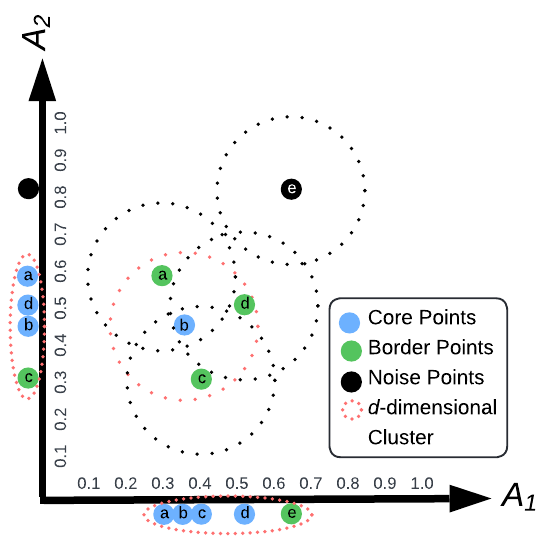
\includegraphics[width=0.33\textwidth]{figures/subclu_cluster.png}\label{fig:subclu_cluster}}~~~~
    \subfloat[][No 2D cluster found after $a$ is moved further up along $A_2$.]{%
        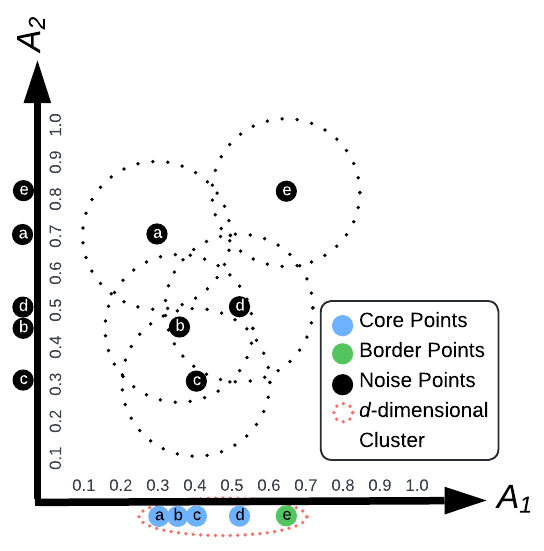
\includegraphics[width=0.33\textwidth]{figures/subclu_no_cluster.png}\label{fig:subclu_no_cluster}}~
    \caption{Illustration of SUBCLU.}
    \label{fig:subclu}
    \vspace*{-0.7cm}
\end{figure}